\begin{ReasoningBox}[title=Quantitative Decision-Making] % 可以通过 title 参数修改标题
    % --- 第一部分：问题描述与图片 ---
    % \begin{minipage}[t]{0.58\textwidth}
    
\textbf{Question:} You are a quantitative analyst backtesting several trading strategies. Here are the five strategies you're evaluating:
        \begin{wrapfigure}{r}{0.5\textwidth}
        \centering
        % wrapfigure 通常顶部会有多余空白，使用负 vspace 向上提，让图片和第一行文字对齐
        \vspace{-20pt} 
        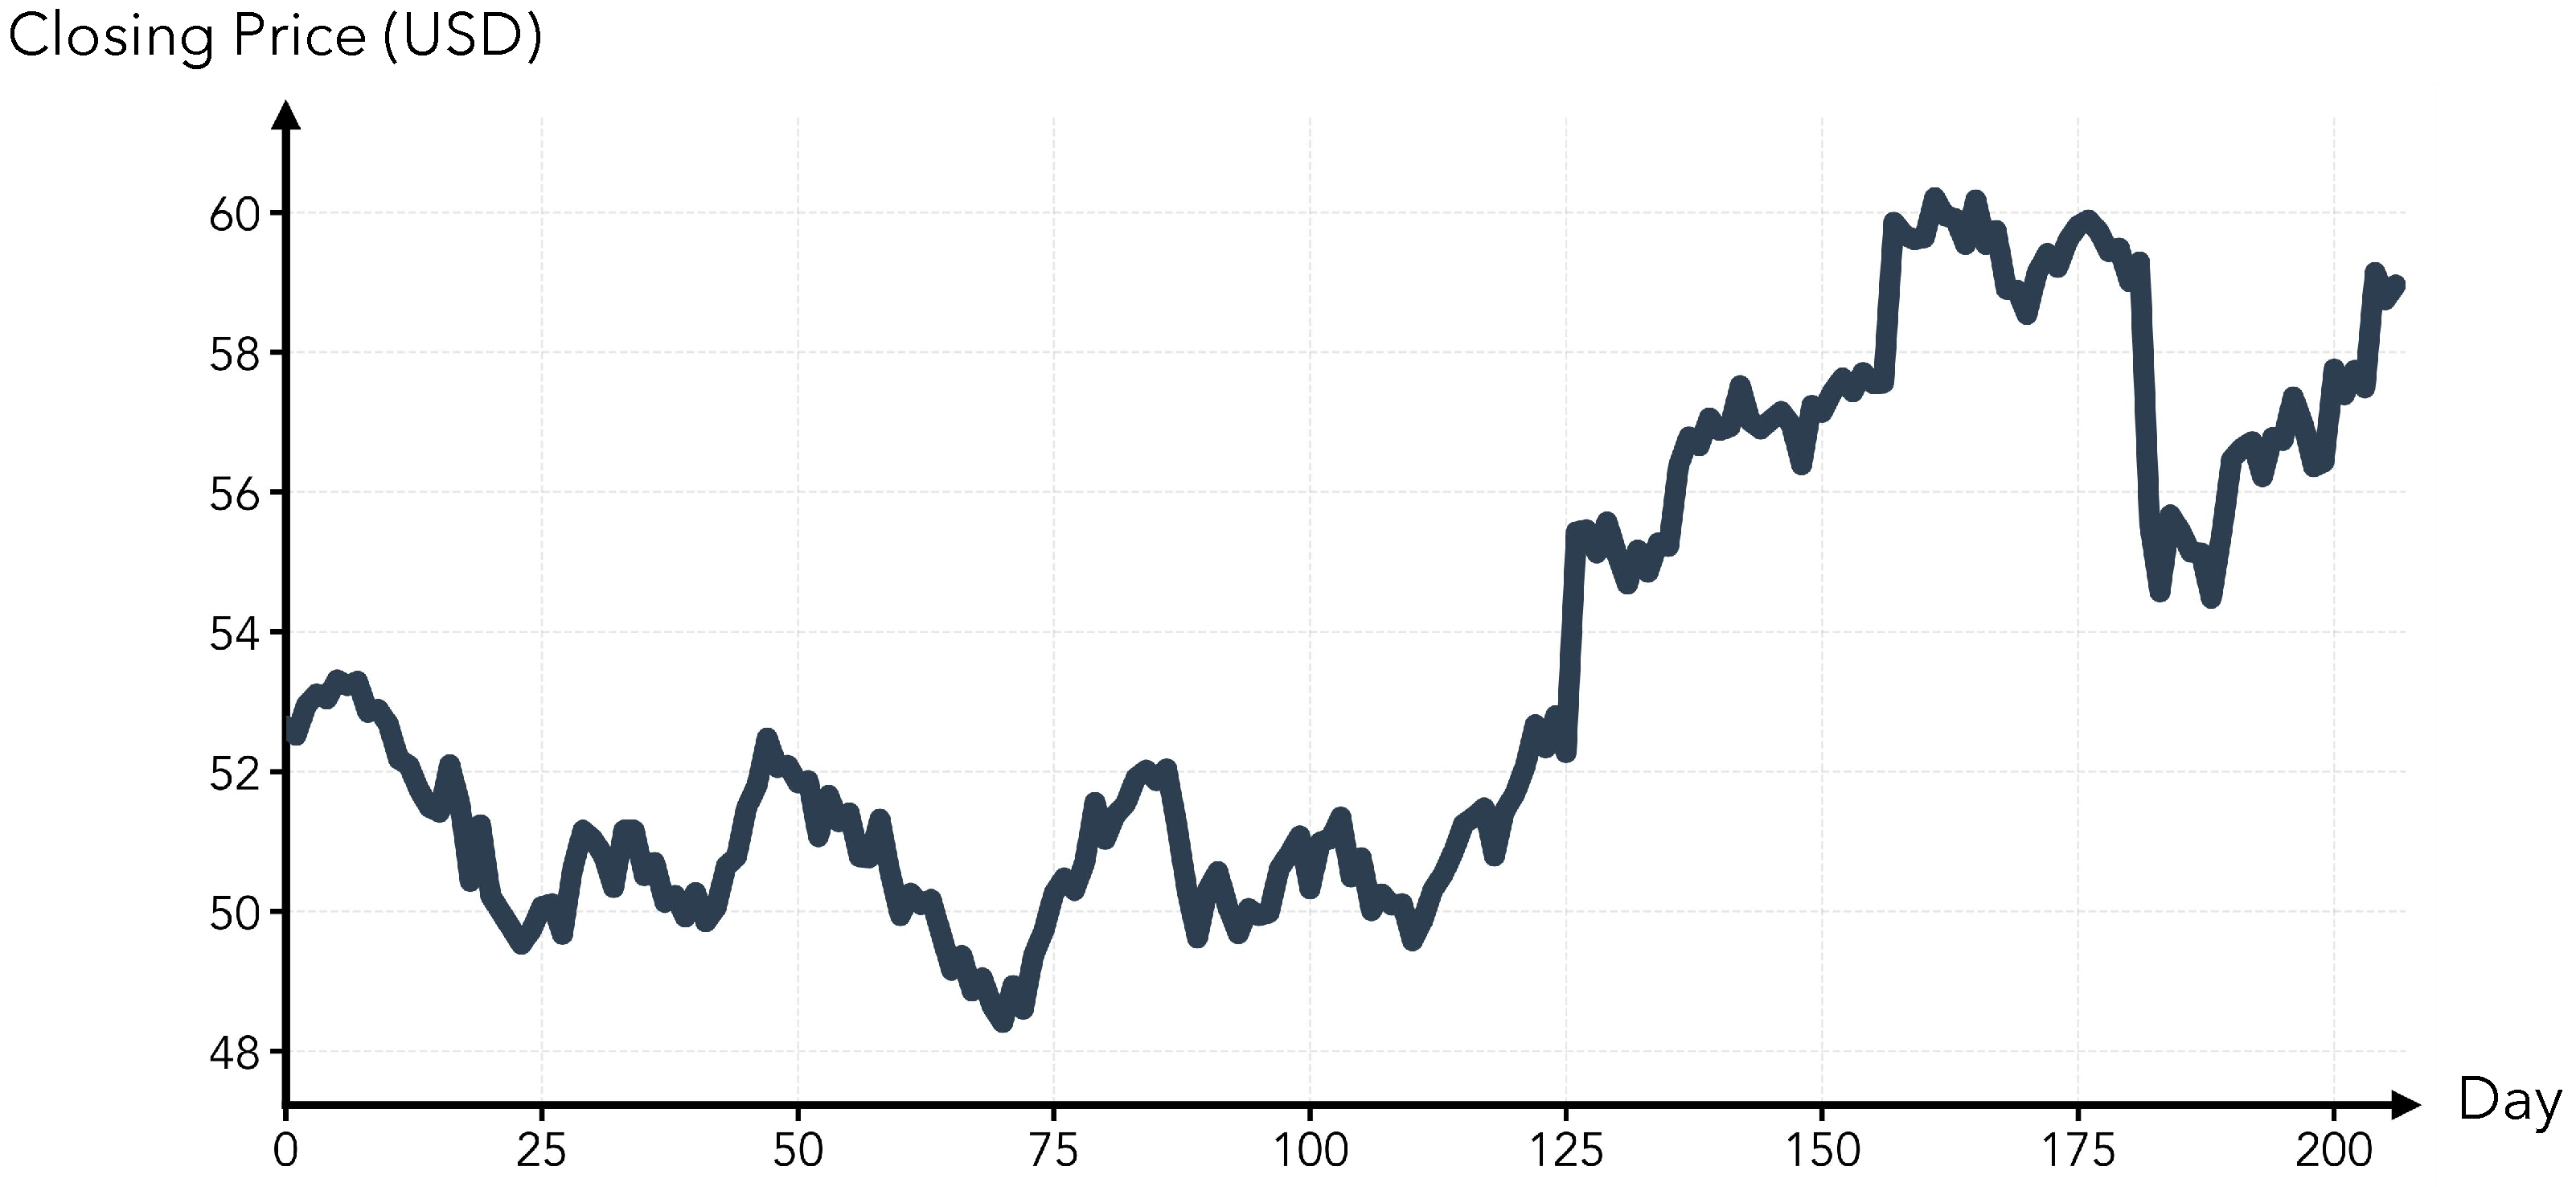
\includegraphics[width=\linewidth]{blocks/sample_cases_success/quantitative.pdf}
        % 调整底部的留白
        \vspace{-20pt}
    \end{wrapfigure}
        (A) SMA Crossover (20/50): Buys when the 20-day moving average crosses above the 50-day moving average, sells when it crosses below.
        (B) MACD (12/26/9): Buys when the MACD line crosses above the signal line, sells when it crosses below.
        (C) RSI (14, 30/70): Buys when RSI falls below 30 (oversold condition), sells when RSI rises above 70 (overbought condition).
        (D) Bollinger Bands (20, $2\sigma$): Buys when price falls below the lower band ($P < \mu - 2\sigma$), sells when price rises above the upper band ($P > \mu + 2\sigma$).
        (E) Buy and Hold: Enters the position at the beginning and holds it for the entire period.
        You have backtested these strategies on the provided price series with an initial capital of \$10,000 and a transaction cost of 0.1\% per trade. Based on the price data provided and standard technical analysis principles, which strategy would you expect to achieve the best Maximum Drawdown (MDD)?
    \vspace{0.5em}

    \textbf{Answer Choices:} \\
    (A) SMA Crossover \\ 
    (B) MACD \\
    (C) RSI \\
    (D) Bollinger Bands\\
    (E) Buy and Hold \\
    \textbf{Correct Answer:} \textcolor{correctgreen}{(D)} \\

\end{ReasoningBox}